\chapter{コメント生成による検出補助}\label{ch:gen_com}
\section{目的}\label{sec:gen_pur}
\label{ch:purpose}
\subsection{対象}
今回対象とする情報は,既にファクトチェックによって真偽が評価されているニュースと,ニュースに対してSNS上で寄せられたコメントである.
詳細な仕様は第\ref{sec:dataset}節で採用したデータセットについて説明する.
真偽はデータセットが採用しているReal・Fakeの2種類である.
また今回対象とする言語は英語である.

実際に実験で使用したReal・Fakeの例が表\ref{tbl:data_example}の通りである.いずれも芸能記事を専門とするファクトチェックプラットフォームであるGossipCopにファクトチェックされ真偽が公表されているものである.
Realの例は俳優のエディ・シブリアンが,女優のリアン・ライムスによる「不健康な行動」に関する告発へ反論する記事\cite{calvario_2017}とコメントを示している.
一方Fakeの例は英国キャサリン妃とメーガン妃は永遠の親友と言えるほど完全に良好な関係ではないかもしれないとする記事\cite{bahou_2018}とコメントを示している.

表\ref{tbl:data_example}のコメントによると,Realのコメントは記事のタイトルを記述した投稿が中心であるが,
Fakeのコメントは特に3件目のように信憑性に疑問を投げかけている.
このことから,コメントを考慮することで,ユーザによる反応から真偽を判断するにあたって有力な手がかりを得られることが予想される.
ただし早期検出に向けて検出実験で使用できるコメントの数が制限されるため,必ずしもそういった情報が得られる訳ではない点に留意が必要である.
\begin{landscape}
\begin{table}[p]
    \centering
    \caption{実験で使用した記事本文の冒頭と実在コメント3件の例.いずれもGossipCopでファクトチェックされている.}
    \label{tbl:data_example}
    \begin{tabularx}{\linewidth}{llX}  \hline
        ラベル & 項目 & 内容 \\ \hline
        \multirow{4}{*}{Real} & 記事                         & \texttt{The drama between Eddie Cibrian and Brandi Glanville continues.  The 43-year-old actor fired back at his ex-wife after she accused Cibrian's wife, LeAnn Rimes, of harassment.  In a statement obtained by ET, Cibrian addresses Glanville's accusations and defends his wife of six years}...\\ \cline{2-3}
                              & \multirow{3}{*}{実在コメント} & \texttt{Eddie Cibrian Responds to Brandi Glanville’s Accusations About LeAnn Rimes https://t.co/QV5UfW7wxm}\\ \cline{3-3}
                              &                             & \texttt{Eddie Cibrian Responds to Brandi Glanville's Accusations About LeAnn Rimes: Eddie Cibrian has broken his… https://t.co/b5dpTHC7Lg \#E\_Online}\\ \cline{3-3}
                              &                             & \texttt{Eddie Cibrian Responds to Brandi Glanville's Accusations About LeAnn Rimes: Eddie Cibrian has broken his silence… https://t.co/vP5aCRjrIF}\\ \hline
        \multirow{4}{*}{Fake} & 記事                         & \texttt{Don’t get us wrong: There’s no truth to those rumors that Meghan Markle and Kate Middleton's relationship is rocky. The two, who are set to be sisters-in-law when Markle marries Prince Harry in May, are certainly amicable. But there’s a difference between being friendly and being} ...\\ \cline{2-3}
                              & \multirow{3}{*}{実在コメント} & \texttt{Prince Harry, Meghan Markle Marriage On The Rocks One Month After Wedding? https://t.co/dKVtv3Ha8O}\\ \cline{3-3}
                              &                             & \texttt{Still, the ``source'' maintains ``things escalated to the point where Meghan was in tears and Harry walked out.'' Pr… https://t.co/RmhtVJHMM}\\ \cline{3-3}
                              &                             & \texttt{For all of these reasons, it’s apparent this article is not credible and shouldn’t be trusted. Prince Harry, Meg… https://t.co/H99mtg1jrl}\\ \hline
    \end{tabularx}
\end{table} 
\end{landscape} 

\newpage
\subsection{達成目標}
本研究は,偽情報の早期検出に向けコメントが少ない状況で検出の実現を目指す.
そのため提案手法が使用する実在コメントは2件に制限し,分類に先立ち記事と実在コメントから想定されるコメントを1件生成し分類に追加入力する.
学習は記事と3件の実在コメントによるコメント生成学習と,記事と2件の実在コメント,そして1件の生成コメントによる分類学習の2回実行する.

本研究を更に発展させると,SNS上で拡散され始めて間もない偽情報を迅速に検出できることに加え,
想定されるコメントを含めてユーザに警告を発することで拡散の抑制へ繋げられる.

\section{手法}\label{cpt:gen_mtd}
\subsection{概要}
\label{sec:method_overall}
この章では,今回の研究で提案する手法の解説を行う.
提案手法は記事コメント生成部分と,記事・実在コメント・生成コメントから真偽分類を行う2つの部分に分けることができる.
記事本文と既存するコメントから,同じ状況で想定されるコメント生成技術を学習する.

提案手法は偽情報を自動で生成するGroverモデルをベースに改良を加えたものである.
GroverモデルはOpenAI GPT-2\cite{Radford_GPT2}から拡張して実装されたものである\cite{Shu:2017:FND:3137597.3137600}.
GPT-2はTransformerをベースにした手法であり,基本的なモデル概略を図\ref{fig:gpt}に引用する\cite{radford2018improving}.
全体のモデル図は図\ref{fig:model}の通りである.

\subsection{モデル定義}
今回扱う記事の集合を 
\begin{equation}
    A = \{a_1, a_2, ..., a_n\}
\end{equation}

とし,それぞれに正解ラベル群 
\begin{equation}
    Y=\{y_1, y_2, ..., y_n\}, y_i = \{0, 1\}
\end{equation}

がつけられているとする.
それぞれの記事$a_i$に対応するラベルが$y_i=0$のときは事実に基づくニュース(Real)とし,
$y_i=1$のときは偽情報(Fake)とする.

一方,コメント集合を
\begin{equation}
    C_A = \{c_{a_1}, c_{a_2}, ..., c_{a_n}\}
\end{equation}
と定義する.
それぞれの記事に寄せられたコメント集合を
\begin{equation}
    C_{a_i} = \{c_{a_{i1}}, c_{a_{i2}}, c_{a_{i3}}\}
\end{equation}
とすることで,
記事$a_i$に対応するコメント集合を定義する.

これより提案するモデルは,コメント生成では$A$と$C_A$を学習の入力に使うことで,
$a_i$と$c_{a_{i1}}, c_{a_{i2}}$から$\hat{c_{a_{i3}}}$を生成するよう訓練する.
また,実際の検出ではコメント$c_{a_{i3}}$を使用せず,生成コメント$\hat{c}_{a_{i3}}$を1件追加した
\begin{equation}
    C'_{a_i} = \{ c_{a_{i1}}, c_{a_{i2}}, \hat{c}_{a_{i3}}\}
\end{equation}
を$C_A$の代わりに$A$とともに検出モデルに入力している.


\subsection{コメント生成}
\label{sec:method_generate}
先行研究により,自然言語文章生成モデルは言語モデルの1つとされており,式\ref{eq:generate}のように
文章$x = \mathrm{w}_1^T = (\mathrm{w}_1, \mathrm{w}_2, ..., \mathrm{w}_T)$
はある単語$\mathrm{w}_t$が生成される前の単語群$ \mathrm{w}_1^{t-1}$による条件付き確率の総積であると定義されている.

\begin{equation}
    \label{eq:generate}
    p(x) = p(\mathrm{w}_1^T) = \prod_{t=1}^{T} p(\mathrm{w}_t|\mathrm{w}_1^{t-1})
\end{equation}

提案モデルによる文章生成の流れは図\ref{fig:method}の通りである.
\ref{sec:generate}節の通り,Groverモデルでは記事を5要素に分けて学習が行われており,
生成及び分類学習において,各要素の始点と終点には開始及び終了トークンが付加されている.
本研究ではこれらの要素を記事本文とそれに寄せられた3件のコメントに置換することで実装する.
Groverモデルに倣い,提案モデルは以下の同時分布として定義する.

\begin{equation}
    \label{eq:joint_distri}
    p(a_i, c_{a_{i1}}, c_{a_{i2}}, c_{a_{i3}})
\end{equation}

コメント生成学習時は,ベースとなったGroverモデルと同様に記事とコメントのセットを2つの集団に分け,無作為に歯抜けにする.
コメントの場合は10\%,記事本文の場合は35\%の確率で歯抜けにしてから一方の集団から学習を行い,もう一方での生成におけるクロスエントロピー誤差を最小化するように訓練される\cite{DBLP:journals/corr/abs-1905-12616}.
提案モデルの目的は記事ではなくSNS上で記事に寄せられたユーザの反応を生成することである.

\subsection{真偽分類}
\label{sec:method_classify}
記事とコメントのセットの末尾にはセットの終端を意味するトークンである\texttt{[CLS]}を追加し,またこのトークンが真偽を分類する際に使われる.
これはGroverモデルがベースとしているGPT-2がとる手法\cite{Radford_GPT2}と同一である.
\texttt{[CLS]}トークンは${a_i, C'_{a_i}}$のセットがもつ特徴が集約されており,
真偽分類モデルが真偽ラベル$\hat{y} = \{0, 1\}$を出力する.
図\ref{fig:process}は実際の記事とコメントのセットを真偽分類するまでの流れを示している.

まず,記事に寄せられたコメント群から実験に使用するため投稿時刻が早い順に3件選出し,コメント生成の学習を行う.
真偽分類する際には,3件の実際に投稿されたコメントから1件削除し生成されたコメントを追加してから真偽の分類を行う.
また,同時に生成コメントを追加しなかった状況で分類を行った際の結果との比較も行った.

\begin{figure}[p]
    \centering
    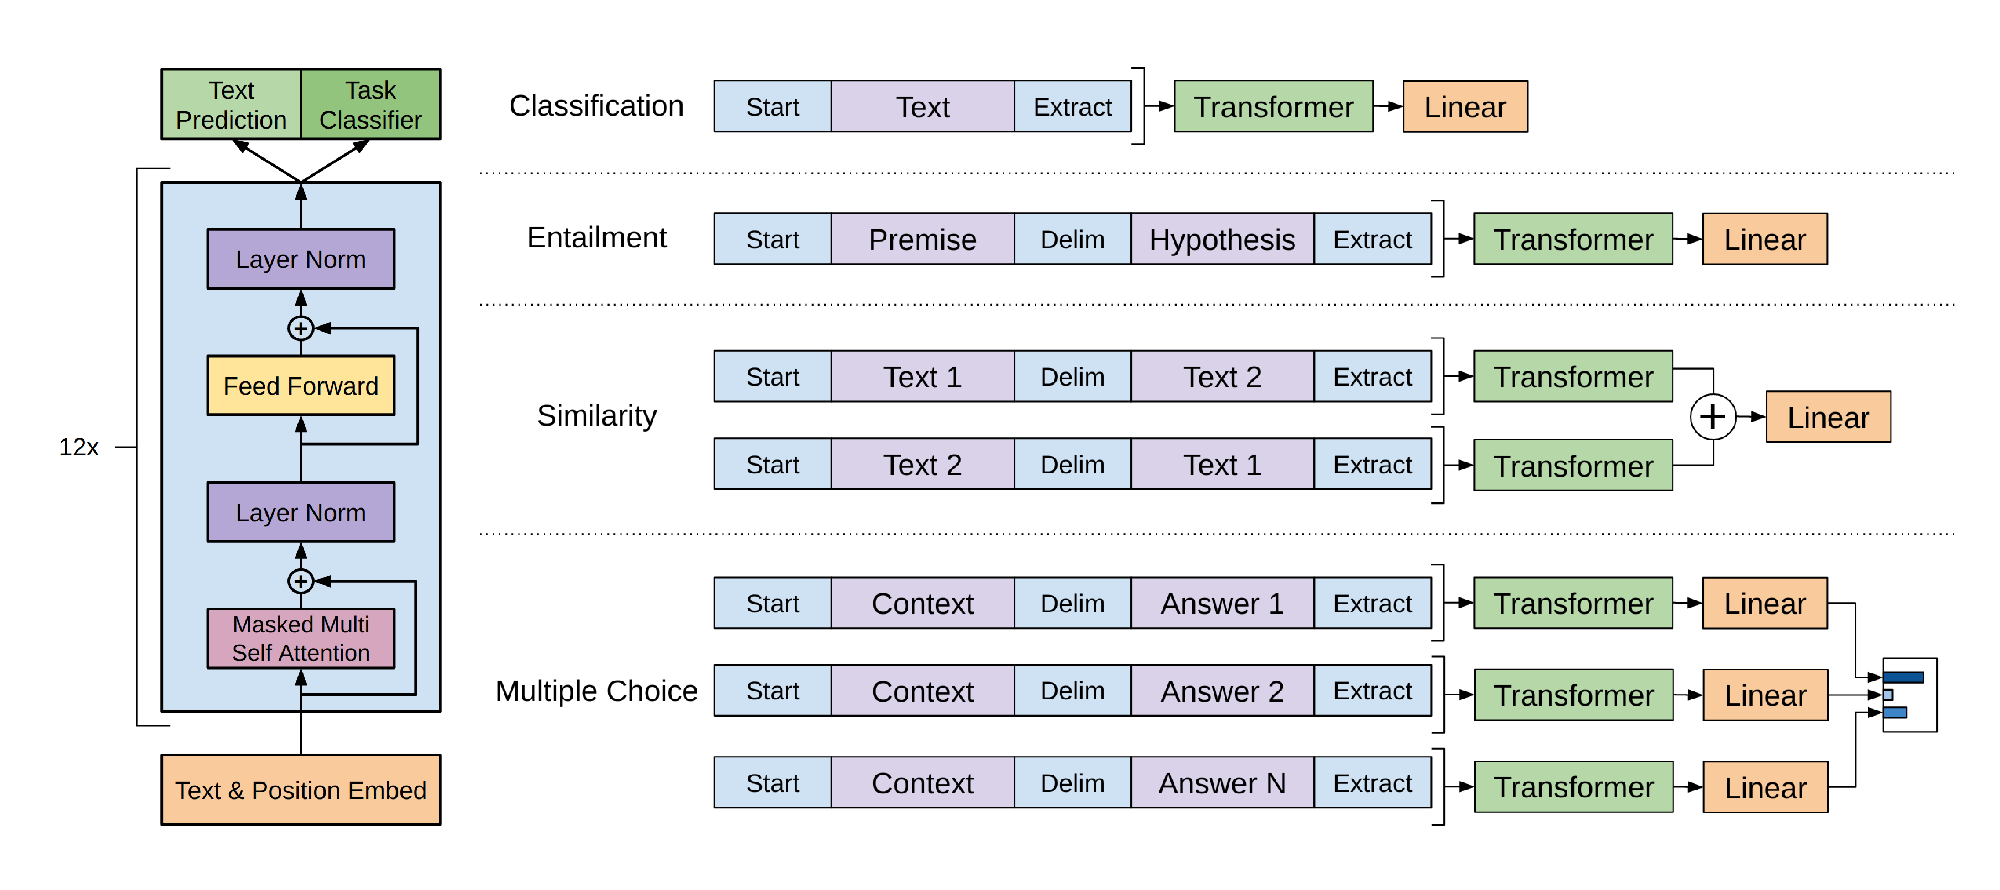
\includegraphics[width=\linewidth,pagebox=cropbox,clip]{figures/fig_gpt.pdf}
    \caption{左: GPT-2のベース手法(GPT)で使われるTransformerのモデル図,右: GPTによる自然言語処理タスクの流れ\cite{radford2018improving}.}
    \label{fig:gpt}
\end{figure}

\begin{figure}
    \centering
    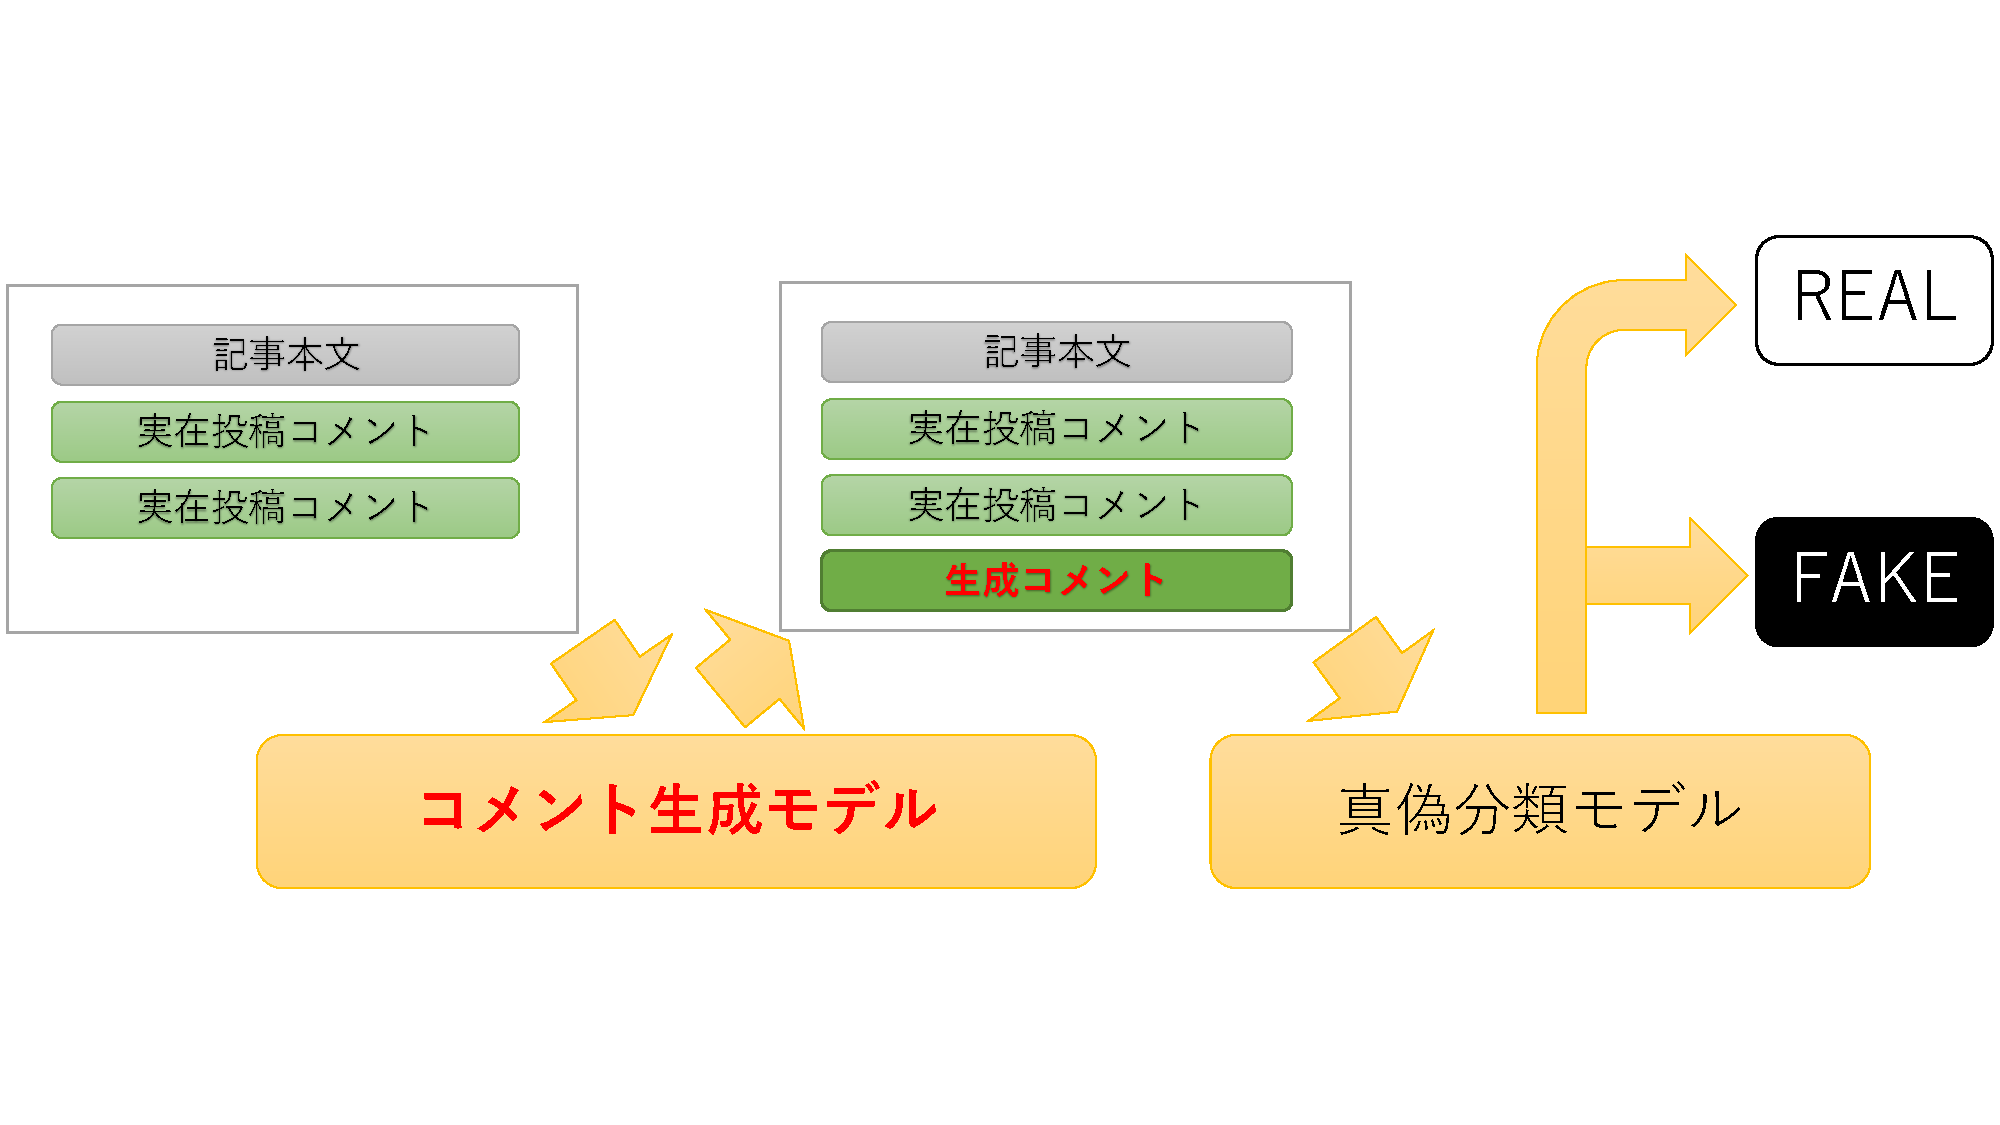
\includegraphics[width=\linewidth,pagebox=cropbox,clip]{figures/fig_model.pdf}
    \caption{モデルの概要図}
    \label{fig:model}
\end{figure}

\begin{figure}[p]
    \centering
    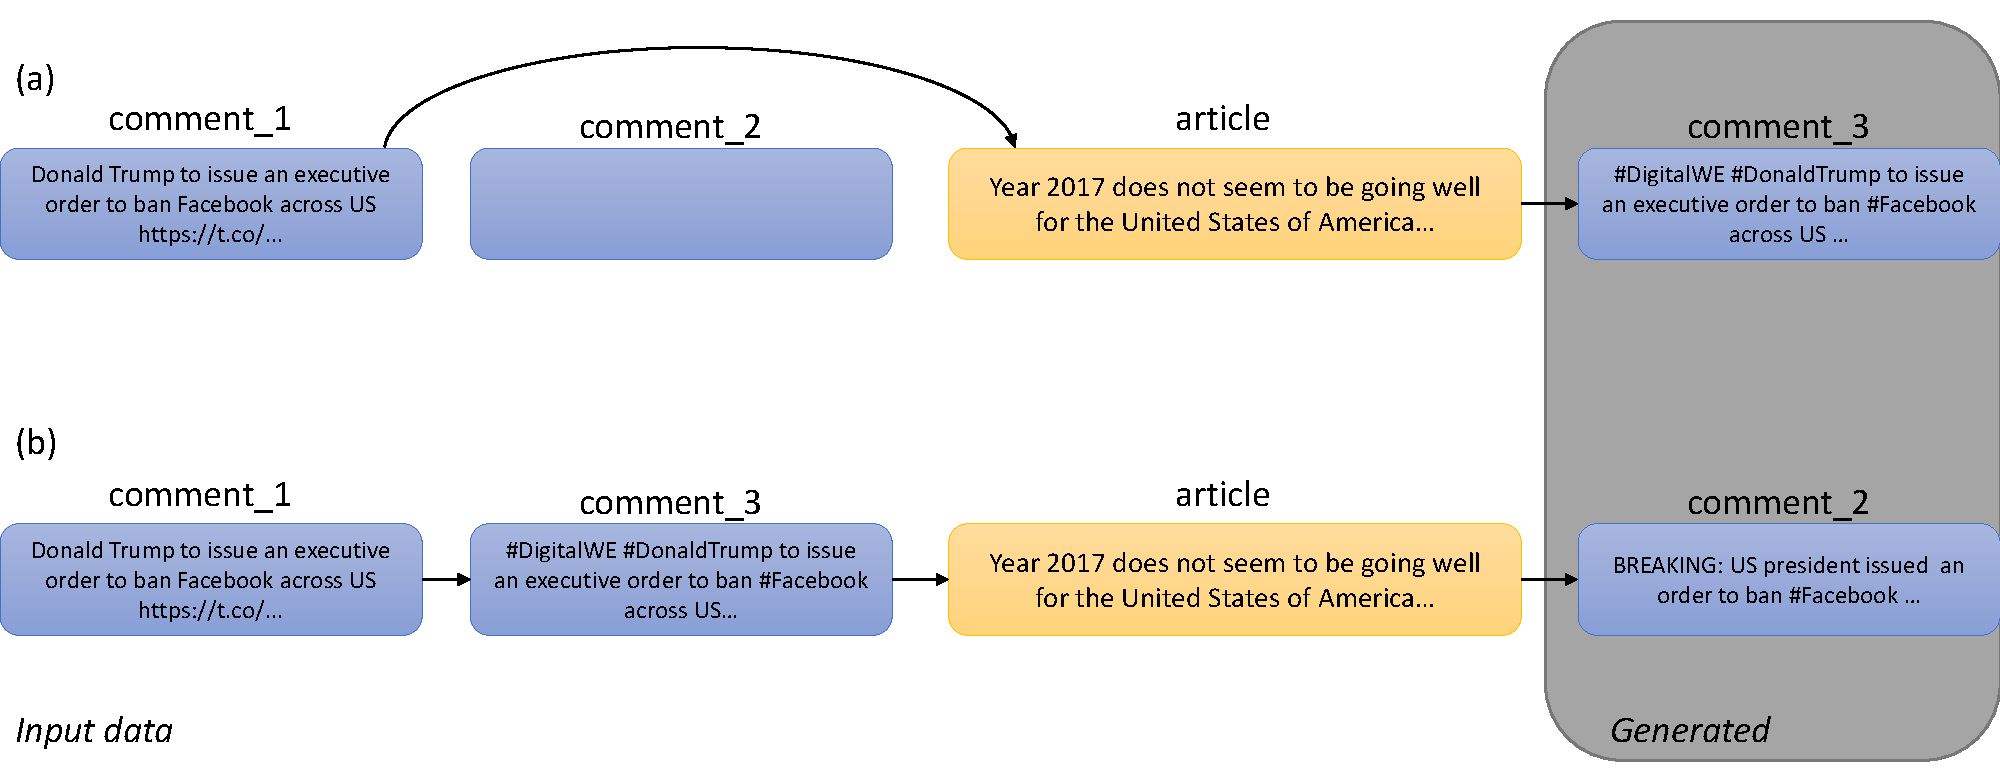
\includegraphics[width=\linewidth,pagebox=cropbox,clip]{figures/fig_method.pdf}
    \caption{
        提案モデルのコメント生成例.
        (a)は記事と1件の実際に寄せられたコメントからコメントを生成している.
        (b)は(a)で生成したコメントを含めた状況で更にコメントを生成している.
    }
    \label{fig:method}
\end{figure}

\begin{figure}[t]
    \centering
    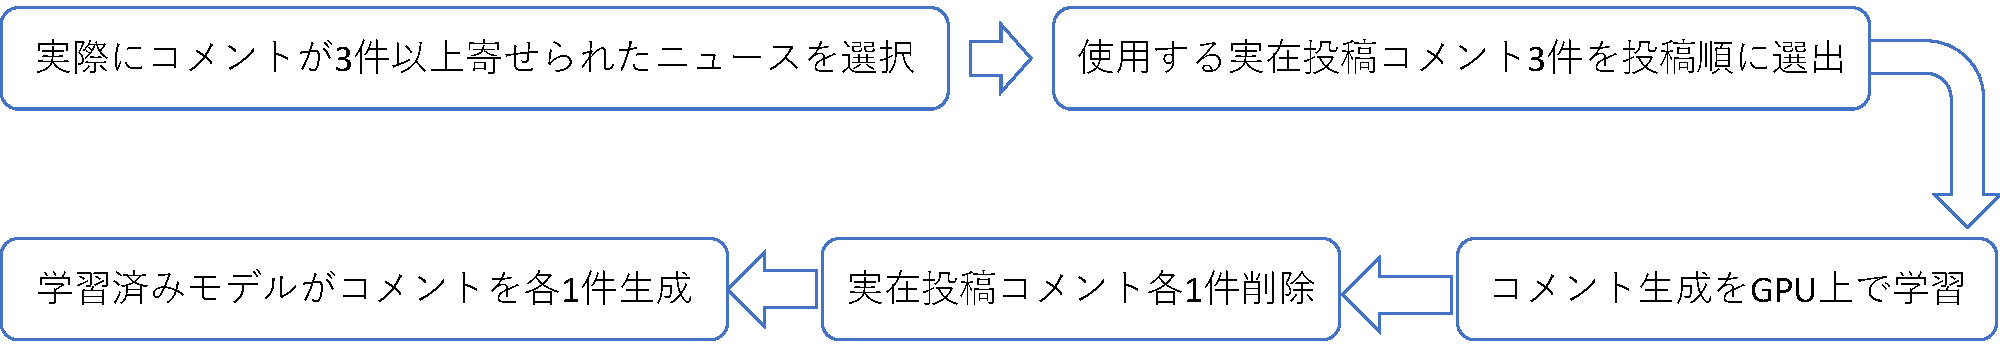
\includegraphics[width=\linewidth,pagebox=cropbox,clip]{figures/fig_process.pdf}
    \caption{実験の流れ}
    \label{fig:process}
\end{figure}

\begin{algorithm}[p]
    \caption{提案モデルが行うコメント生成学習の流れ}
    \label{alg:generate}
    \begin{algorithmic}[1]
%        \REQUIRE $A = \{a_1, a_2, ..., a_n\}, C_A = \{c_{a_1}, c_{a_2}, ..., c_{a_n}\}$
%        \ENSURE $\hat{c_{a_{i3}}}$
        \Procedure{Prepare-Generate}{$A, C_A$}
            \For {$i=1 \, \ldots \, N$}
                \State{articleRand $=$ a random float number between 0 to 1}
                \State{commentRands $=$ three random float numbers between 0 to 1}
                \If{articleRand $\leq 0.35$}
                    \State{make $a_i$ empty}
                \EndIf
                \For {$j=1 \, \ldots \, 3$}
                    \If{articleRand[j] $\leq 0.1$}
                        \State{make $c_{a_{ij}}$ empty}
                    \EndIf
                \EndFor
            \EndFor
        \EndProcedure

        \Procedure{Generate-Training}{$A, C_A$}
            \For {$i=1 \, \ldots \, \mathrm{maxEpoch}$}
                \For{$i=1 \, \ldots \, N$}
                    \While{empty element in $\{a_i, c_{a_i}\}$}
                        \State{Fill an element which is empty in $\{a_i, c_{a_i}\}$}
                    \EndWhile
                \EndFor
            \EndFor
        \EndProcedure
    \end{algorithmic}
\end{algorithm}

\begin{algorithm}
    \caption{提案モデルが行うコメント生成を伴う真偽分類を行う際の流れ}
    \label{alg:classify}
    \begin{algorithmic}[1]
        \Procedure{Classify}{$A, C'_A$}
            \For{$i=1 \, \ldots \, N$}
                \State{Add \texttt{[CLS]} in tail of set ($a_i, C'_{a_i}$)}
                \State{\texttt{[CLS]} has features of set ($a_i, C'_{a_i}$)}
                \State{Classifier outputs label $\hat{y}$ from the \texttt{[CLS]}}
            \EndFor
        \EndProcedure
    \end{algorithmic}
\end{algorithm}


\section{実験}\label{sec:gen_exp}
この章では,提案手法の有効性を検証するために行った実験と結果について記述する.

\subsection{データセット}
\label{sec:dataset}
記事とそれに寄せられたコメントをもつデータセットとしてFakeNewsNet\cite{Shu2018FakeNewsNetAD}を採用した.
これはファクトチェックプラットフォームであるPolitiFact(政治ニュース専門)とGossipCop(芸能ニュース専門)によりファクトチェック(真偽ラベル付けも兼ねる)が行われた記事の内容と,それにTwitter(取得当時)上で寄せられたコメント投稿等を持っている.

実験に先立ち,今回のモデルの構造上少なくとも3件コメントが寄せられているニュースである必要がある他,そのいずれも英文で書かれたコメントである記事とコメントのセットを選出した.
表\ref{tbl:dataset}の通り今回,PolitiFactを使用した実験ではReal・Fakeで各200セット,GossipCopでは毎に2000セット使用した.

\begin{table}[p]
    \caption{実験で使用したラベル毎のデータセット内容.記事数・コメント数はRealとFakeともに同数である.}
    \label{tbl:dataset}
    \centering
    \begin{tabular}{lcc}
        \hline
        ファクトチェックプラットフォーム     & 記事数 & コメント数 \\ \hline
        PolitiFact & 200   & 600   \\
        GossipCop  & 2000  & 6000  \\ \hline
    \end{tabular}
\end{table}

\subsection{実験内容}
\label{sec:exp_contents}
今回実験を2種類行った.

\subsubsection{真偽分類成績調査}
生成コメントを追加することによって真偽分類の傾向に変化がみられるか調べた.
比較対象として2件ともにデータセットがもつコメントを使用したものと,コメントを使わず記事内容のみで真偽分類したものを用意した.
この実験にはセット数が多く汎化性が高いGossipCopにファクトチェックされた記事を採用した.

\subsubsection{生成コメント傾向調査}
生成されたコメントは真偽でどのような単語の傾向が現れるか調べた.
傾向の違いを調べることによって,拡散の初期段階において読者が記事をどう捉えているのか知ることができる.
この実験はセット数が少ないが社会に与える影響が芸能に比べて大きくなりやすい政治ニュースを扱うPolitiFactにファクトチェックされた記事を採用した.

実際に生成されたコメントに対して,すべてアルファベットを小文字にした上で単語ごとの出現回数と出現確率を算出した.
また,算出するにあたって記号(クォーテーションやピリオド,コンマなど)やURLの削除を行ったほか,``a''や``is''といったストップワードはNLTK\cite{bird-loper-2004-nltk}が提供するメソッドを使用して除外した.
なお,コメントの収集元がTwitterであることから,Twitter独自の用法をもつ記号(ハッシュタグ\#やメンション@),またコロンは例外として除外しなかった.

\section{実験結果}
\label{sec:result}
GossipCopを対象とした真偽分類実験結果は表\ref{tbl:classify_results}の通りである.
提案モデルは再現率において全体ベストとなったものの,適合率においては生成モデルを使わない方が優秀であることが読み取れる.

分類において生成コメントの有無によって真偽が覆った回数も調査した.その結果が表\ref{tbl:reversed}の通りである.

また,表\ref{tbl:generated_comments}の生成されたコメントの例のように,生成コメントには文法面にさらなる改善の必要性が残された.

一方,PolitiFactを対象とした生成コメントには,以下のような傾向が見られた.
\begin{itemize}
    \item 真偽問わず最も頻度が高い単語は``via''であり,真偽全体の単語のうち約1.5\%を占めた.
    \item それに続いて``trump''と``obama''が続いたが,いずれも割合は1\%を下回った.
\end{itemize}

これに加えて,真偽における傾向差として以下の違いが見られた.

\begin{itemize}
    \item ``via''は真偽単独で見てもそれぞれで最も高い頻度で生成されていた.
    \item 偽における``via''の生成頻度は正しい場合に比べて約2倍であり,その差は約0.9ポイントと偽頻出上位10単語中最多だった.
    \item ``breaking:''という単語が``via''に次いで2番目に頻度の差が高い単語であり,その差は0.7ポイントだった.
\end{itemize}


\begin{table}
    \renewcommand{\arraystretch}{1.3}
    \caption{分類成績}
    \label{tbl:classify_results}
    \centering
    \begin{tabular}{lccc}
        \hline
        入力データ           & 適合率 & 再現率 & F値 \\ \hline
        記事本文のみ         & 0.647     & 0.615  & 0.631    \\
        + 実在コメント2件  & \textbf{0.774}     & 0.635  & \textbf{0.698}    \\
        + 生成コメント1件 & 0.626     & \textbf{0.695}  & 0.659    \\ \hline
    \end{tabular}
\end{table}

\begin{table}
    \caption{生成コメントの追加により真偽が覆った件数}
    \label{tbl:reversed}
    \centering
    \begin{tabular}{llccc} \hline
        正解ラベル & 覆ったパターン & 覆った件数 & 覆らなかった件数 & 覆った割合[\%]\\ \hline
        \multirow{2}{*}{Real} & Real $\rightarrow$ Fake & 60 & 103 & 37\\
                              & Fake $\rightarrow$ Real & 14 & 23 & 38\\ \hline
        \multirow{2}{*}{Fake} & Real $\rightarrow$ Fake & 35 & 38 & 48\\
                              & Fake $\rightarrow$ Real & 23 & 104 & 18\\ \hline
    \end{tabular}
\end{table}

\begin{table}
    \caption{FakeとRealにおける生成コメント内の頻出単語一覧}
    \label{tbl:frequency}
    \centering
    \begin{tabular}[]{llc}\hline
        順位&Realの頻出単語&出現率[\%]\\ \hline
        \rownumber & via & 1.07 \\
        \rownumber & trump & 0.69 \\
        \rownumber & obama & 0.55 \\
        \rownumber & new & 0.41 \\
        \rownumber & national & 0.41 \\
        \rownumber & said & 0.38 \\
        \rownumber & news & 0.38 \\
        \rownumber & clinton & 0.31 \\ \hline
    \end{tabular}
    \quad
    \begin{tabular}[]{llc}\hline
        順位&Fakeの頻出単語&出現率[\%]\\ \hline
        \rownumber & via & 2.03 \\
        \rownumber & trump & 0.97 \\
        \rownumber & \textbf{breaking:} & 0.92 \\
        \rownumber & obama & 0.87 \\
        \rownumber & president & 0.73 \\
        \rownumber & united & 0.53 \\
        \rownumber & states & 0.44 \\
        \rownumber & years & 0.39 \\ \hline
    \end{tabular}
        
\end{table}

\begin{landscape}
\begin{table}[p]
    \caption{実際に生成されたコメントの一部の冒頭."\textbackslash n"は改行記号である.}
    \label{tbl:generated_comments}
    \centering
    \begin{tabular}{ll}
        \hline
        ラベル & 生成コメント(冒頭) \\ \hline
        Real & \texttt{talks to theWa at theus\textbackslash n�, Read,rin would Huck Randall. didn}...\\
        Real & \texttt{accuracy!co/g Making, single change of Wyn, the fell Featuresogue,}...\\
        Real & \texttt{Vi thepressBir 143 Introdu sting Sullivan remarksregnancy prof}...\\
        Real & \texttt{she theheyhl height backyardGame his-Whereas to peach THRrd, go}...\\
        Real & \texttt{gory for Emil-----][PU Adidasolan Song and Patrick.itans.\textbackslash n\textbackslash n}...\\ \hline
        Fake & \texttt{guest Chelsea1p henEach psychologicalZEinspired second resort}...\\
        Fake & \texttt{eeleurg, Rum rates as aHS Army to week it3 transplant nomination KnW}... \\
        Fake & \texttt{View was22 the Ridge caval Shar silicone Copyright warm Yourhm Had,}...\\
        Fake & \texttt{\textbackslash n\textbackslash n\textbackslash n\textbackslash n\textbackslash n\textbackslash nThe756 anticipating appetite sungIMels sightings in}...\\
        Fake & \texttt{s tagging going.What back advocate Rum to- lonelymentation her tie}...\\ \hline
    \end{tabular}
\end{table}
\end{landscape}

\section{考察}\label{sec:gen_evl}
\subsection{真偽分類成績指標}
\label{sec:classify_index}
\cref{tbl:classify_results}が真偽分類を行った結果である.
記事のみから分類した場合と,記事に加えてコメントを入力に含めた場合では,コメントを含めると分類成績に改善がみられることがわかる.
このことから,記事単体に加えて読者が送ったコメントが正確な真偽分類に貢献することが示されている.

また実在コメントのみ入力した場合と,加えて提案モデルによって生成したコメントを含めた場合より,提案モデルは再現率は全体ベストを示したものの,適合率に大きな課題を残した.
これは提案モデルがソーシャルコンテキストが制限されている状況でも,単純に真偽分類を行うより多くの偽情報の検出ができることを意味する.

\subsection{真偽分類傾向差の比較}
\label{sec:classify_trend}
実際真偽分類の傾向を調べるため,Realを0,Fakeを1とした分類の平均値を調べた.
その結果生成コメントがない場合は0.41,ある場合は0.55で,対応ありt検定の結果$p<0.05$だった.
このことから,生成コメントによってFakeを多く分類する傾向の有意差がみられた.
また\cref{tbl:reversed}より,生成コメントがない場合でRealと判定していた検出モデルが,
生成コメントの追加によってFakeへ判断が95件覆っていることが読み取れる.
内訳では95件中35件が正解ラベルがFakeである偽情報であることと,
正解ラベルFakeのうち23件のみ生成コメントでFakeからRealに覆っていることから,
生成コメントの追加によって検出モデルがRealと誤って判断しにくくなったことが伺える.
このことは正解ラベル毎に生成コメントによって出力ラベルが覆った件数を生成コメントの出力ラベル毎の件数で割った割合からも,
特に正解ラベルFakeの場合においてモデルが騙されにくくなったとみられる.
一方残りの60件はRealに対してFakeと誤った判断へ誘導しているため,
生成コメントによる適合率の減少を誘発していると考えられる.

また生成コメントなしの出力ラベルに対して,
真偽が覆った件数を、元々の出力ラベル毎に分けた件数分無作為にラベルを反転させた時の
分類指標を調べたところ,適合率は0.486, 再現率は0.390, F値は0.429といずれの手法を大幅に下回っていた.

\cref{sec:classify_index}と併せると,この傾向はファクトチェックが必要なニュースを探す際に役立つことを示唆している.
ただし適合率が低く他のモデルより多く正しいニュースを偽情報として誤って検出するため,改善が求められる.
今後は,より多くのデータセットを用いた場合に傾向が変化するか調べる必要がある.

\subsection{単語生成傾向}
コメント生成の傾向から,提案モデルは入力されたニュース記事が扱うトピックの学習に成功したように見える.
生成されたコメントの多くが政治的内容を含むものが多かった理由として,データセットが扱う内容の影響を受けたことが考えられる.

生成コメントの中で興味深い単語は``breaking:''である.
この単語は偽情報に寄せられたコメントとして生成されていた.
本研究と同じくコメントとして尤もらしい単語を生成するTCNN-URG \cite{ijcai2018-533}でも,
偽を示すシグナルとして``!''や``?'',そして``false''が報告されていたが,``breaking:''は報告されていなかった.
よって,この``breaking:''も偽情報を示す重要なシグナルである可能性がある.

\subsection{生成コメントの内容}
生成されたコメントは文法面に改善点が残されているが,これはデータセットの規模不足が原因として考えられる.
Groverモデルは120GBにも及ぶニュースデータセットから訓練されていた \cite{DBLP:journals/corr/abs-1905-12616}ことも考慮すると,
改善のためにはさらなる追加データを収集する必要がある可能性が示されている.

もう1つの文法面の完成度改善に向けて考えられる対策として,ベースとなる手法の変更も考えられる.
\cref{sec:method_overall}の通り,提案手法はGPT-2から発展させたものである.
現在ではGPT-2の発展型にあたるGPT-3\cite{brown2020language}やGPT-4 \cite{openai2023gpt4}を始めとする自然言語処理モデルの進歩が著しいため,
ベースとなるモデルを変更することでより自然なコメント生成が可能となる可能性がある.
